\chapter{Grafos}

A lo largo de la memoria mencionamos varias veces la palabra grafo. En este anexo introduciremos todos los conceptos relacionados con grafos y algunos ejemplos de los tipos de grafos más conocidos. El primero en hablar de grafos fue Euler en el año 1736 cuando resolvió el problema matemático de los siete puentes de Königsberg (la formulación y solución al problema se puede encontrar en \cite{refpuentes}) que dio origen a la teoría de grafos.\\

Pueden existir variantes de algunas de las definiciones que usaremos a continuación, la mayoría de las usadas han sido traducidas de \cite{librografos}.

\section{Conceptos básicos}

\begin{defi} 
	Un grafo (o grafo no dirigido) $G$ es un par ordenado $G=(V,E)$, donde:
	\begin{itemize}
		\item $V$ es un conjunto de vértices o nodos, y
		\item $E$ es un conjunto de aristas o arcos, que relacionan estos nodos.
	\end{itemize}
\end{defi}

Una arista que une dos nodos $v_{1},v_{2} \in V$ se denota como $v_{1}v_{2}$ o $v_{2}v_{1} \in E$. Cuando el nodo origen y el destino de una arista son el mismo estaremos hablando de bucles. Decimos que dos aristas son paralelas cuando ambas aristas relacionan el mismo par de vértices. Dos aristas son adyacentes si tienen un vértice en común, y dos vértices son adyacentes si existe una arista que los une.

\begin{defi} 
	El orden de un grafo $G$ es el número de vértices de $G$, es decir, $|V|$.
\end{defi}

Nos interesará estudiar los grafos finitos, cuando $|G|< \infty$, ya que muchos de los resultados sobre grafos no se pueden aplicar a grafos infinitos.

\begin{defi} 
	El grado de un nodo $v \in V$ se define como el número de aristas que lo tienen como extremo.
\end{defi}

\newpage

\begin{ejem} 
	En la figura \ref{fig:graph} se muestra un grafo donde $ V = \{1,2,3\} \text{  y  } E = \{12,23\} $.
\end{ejem}

\begin{figure}[H]
	\centering
	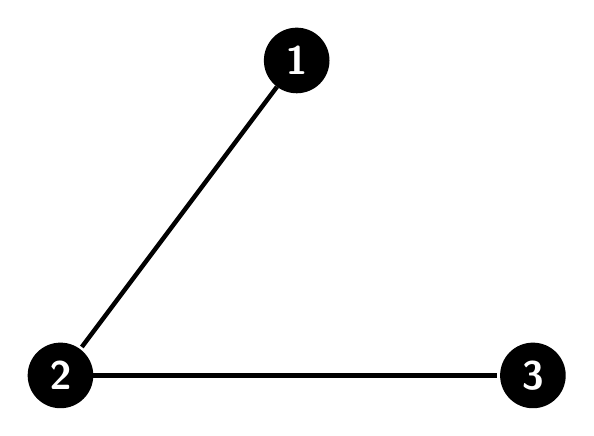
\begin{tikzpicture}[shorten >=1pt, auto, node distance=3cm, ultra thick]
	\tikzstyle{node_style} = [circle,draw=black,fill=black,font=\sffamily\Large\bfseries,text=white]
	\tikzstyle{edge_style} = [draw=black, line width=2, ultra thick]
	\node[node_style] (v1) at (0,2) {1};
	\node[node_style] (v2) at (-3,-2) {2};
	\node[node_style] (v3) at (3,-2) {3};
	\draw[edge_style] (v1) edge (v2);
	\draw[edge_style] (v2) edge (v3);
	\end{tikzpicture}
	\caption{Ejemplo de grafo.}
	\label{fig:graph}
\end{figure}

El orden del grafo es 3. \\
El grado de cada uno de los nodos es $$g(1)=g(3)=1$$  $$g(2)=2.$$\\
\qed

\begin{defi} 
	El grafo complementario de $G$ se denota $\bar{G}$ y tiene el mismo conjunto de vértices que $G$, pero su conjunto de aristas son todas aquellas que unen los vértices que no están unidos en $G$.
\end{defi}

\begin{ejem} 
	En la figura \ref{fig:graphcomplementario} se muestra el grafo complementario del de la figura \ref{fig:graph}.
\end{ejem}

\begin{figure}[H]
	\centering
	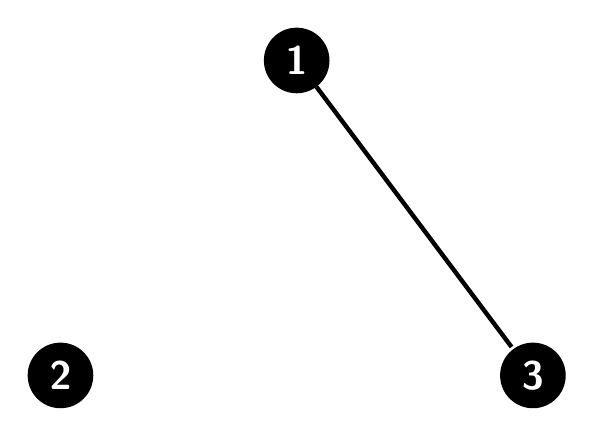
\begin{tikzpicture}[shorten >=1pt, auto, node distance=3cm, ultra thick]
	\tikzstyle{node_style} = [circle,draw=black,fill=black,font=\sffamily\Large\bfseries,text=white]
	\tikzstyle{edge_style} = [draw=black, line width=2, ultra thick]
	\node[node_style] (v1) at (0,2) {1};
	\node[node_style] (v2) at (-3,-2) {2};
	\node[node_style] (v3) at (3,-2) {3};
	\draw[edge_style] (v1) edge (v3);
	\end{tikzpicture}
	\caption{Ejemplo de grafo complementario.}
	\label{fig:graphcomplementario}
\end{figure}

\qed

\begin{defi} 
	Dado un grafo $G=(V,E)$. Un camino de $v_{0}$ a $v_{n}$ es una sucesión de aristas $e_{1},e_{2},\dots,e_{n}$ de la forma $e_{1}=v_{0}v_{1}$, $e_{2}=v_{1}v_{2}$, $\dots$, $e_{n}=v_{n-1}v_{n}$, donde $v_{0}$ es el inicio del camino, $v_{n}$ es el fin del camino y la longitud del camino viene dada por el número de aristas de éste.
\end{defi}

\section{Tipos de grafos}

Existen multitud de tipos de grafos diferentes. Ya hemos mencionado algunos como los grafos no dirigidos, los grafos finitos y los infinitos. Vamos a presentar algunos tipos más:
\begin{itemize}
	\item Grafo nulo: es un grafo cuyos vértices no tienen ninguna arista que los una.
	
	\begin{figure}[H]
		\centering
		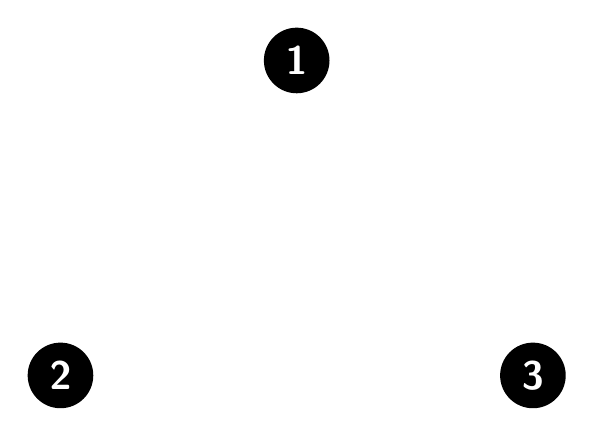
\begin{tikzpicture}[shorten >=1pt, auto, node distance=3cm, ultra thick]
		\tikzstyle{node_style} = [circle,draw=black,fill=black,font=\sffamily\Large\bfseries,text=white]
		\tikzstyle{edge_style} = [draw=black, line width=2, ultra thick]
		\node[node_style] (v1) at (0,2) {1};
		\node[node_style] (v2) at (-3,-2) {2};
		\node[node_style] (v3) at (3,-2) {3};
		\end{tikzpicture}
		\caption{Ejemplo de grafo nulo.}
		\label{fig:grafonulo}
	\end{figure}
	
	\item Grafo simple: es un grafo que no posee bucles ni aristas paralelas. Los ejemplos que hemos visto hasta ahora son todos grafos simples.
	\item Multigrafo: $G$ es un multigrafo si y solo si no es simple, es decir, tiene bucles y/o aristas paralelas.
	
	\begin{figure}[H] 
		\centering
		\tikzset{me/.style={to path={
			\pgfextra{
				\pgfmathsetmacro{\startf}{-(#1-1)/2}  
				\pgfmathsetmacro{\endf}{-\startf} 
				\pgfmathsetmacro{\stepf}{\startf+1}}
			\ifnum 1=#1 -- (\tikztotarget)  \else
			\foreach \i in {\startf,\stepf,...,\endf}
			{
				(\tikztostart) parabola[bend pos=0.5] bend +(0,0.4*\i)  (\tikztotarget)
			}
			\fi   
			\tikztonodes
		}}}  			
		
		\begin{tikzpicture}[shorten >=1pt, auto, node distance=3cm, ultra thick,every loop/.style=]
			\tikzstyle{node_style} = [circle,draw=black,fill=black,font=\sffamily\Large\bfseries,text=white]
			\tikzstyle{edge_style} = [draw=black, line width=2, ultra thick]
			\node[node_style] (v1) at (0,2) {1};
			\node[node_style] (v2) at (-3,-2) {2};
			\node[node_style] (v3) at (3,-2) {3};
			\draw[edge_style] (v1) edge (v2);
			\draw[thick] (v2) edge[me=5] (v3); 
			\path[thick] (v1) edge [loop above] ();
			\path[thick] (v2) edge [loop left] ();
			\path[thick] (v3) edge [loop right] ();
		\end{tikzpicture}
		\caption{Ejemplo multigrafo.}
	\end{figure}
	
	\newpage
	
	\item Grafo completo: es un grafo simple que cumple que para cada par de vértices del grafo existe una arista que los une, es decir, contiene todas las aristas posibles.
	
	\begin{figure}[H]
		\centering
		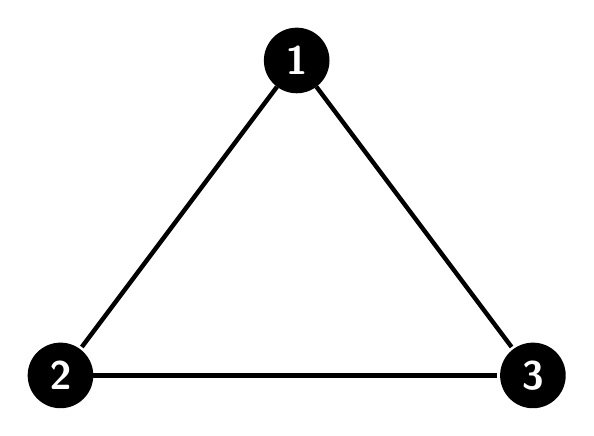
\begin{tikzpicture}[shorten >=1pt, auto, node distance=3cm, ultra thick]
		\tikzstyle{node_style} = [circle,draw=black,fill=black,font=\sffamily\Large\bfseries,text=white]
		\tikzstyle{edge_style} = [draw=black, line width=2, ultra thick]
		\node[node_style] (v1) at (0,2) {1};
		\node[node_style] (v2) at (-3,-2) {2};
		\node[node_style] (v3) at (3,-2) {3};
		\draw[edge_style] (v1) edge (v2);
		\draw[edge_style] (v1) edge (v3);
		\draw[edge_style] (v2) edge (v3);
		\end{tikzpicture}
		\caption{Ejemplo de grafo completo.}
		\label{fig:grafocompleto}
	\end{figure}
	Nótese que cuando tenemos el mismo conjunto de vértices $V$, el grafo nulo y el grafo completo son complementarios. Por ejemplo, el grafo de la figura \ref{fig:grafonulo} y el de la figura \ref{fig:grafocompleto} son complementarios.

	\item Grafo regular: es un grafo en el que todos los nodos tienen el mismo grado. Por ejemplo el grafo de la figura \ref{fig:grafocompleto} es un grafo regular.

	\item Grafo conexo: es un grafo que cumple que para cada par de nodos existe al menos un camino que los une. La mayoría de grafos vistos hasta ahora son conexos. El grafo de la figura \ref{fig:graphcomplementario} es un grafo no conexo ya que el vértice 2 no tiene ningún camino que lo una a 1 y 3.
	
	\item  Árbol: son grafos que conectan todos los vértices utilizando el menor número posible de aristas. Tienen $n$ nodos y $n-1$ aristas.
	
	\begin{figure}[H]
		\centering
		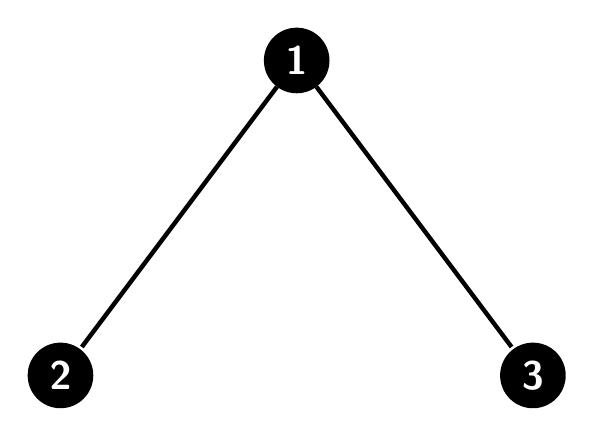
\begin{tikzpicture}[shorten >=1pt, auto, node distance=3cm, ultra thick]
		\tikzstyle{node_style} = [circle,draw=black,fill=black,font=\sffamily\Large\bfseries,text=white]
		\tikzstyle{edge_style} = [draw=black, line width=2, ultra thick]
		\node[node_style] (v1) at (0,2) {1};
		\node[node_style] (v2) at (-3,-2) {2};
		\node[node_style] (v3) at (3,-2) {3};
		\draw[edge_style] (v1) edge (v2);
		\draw[edge_style] (v1) edge (v3);
		\end{tikzpicture}
		\caption{Ejemplo de árbol.}
	\end{figure}

	\newpage

	\item Grafo dirigido: es un tipo de grafo en el cual las aristas tienen una dirección definida, tienen un nodo de inicio y uno de fin. En un grafo dirigido las aristas $v_{1}v_{2}$ y $v_{2}v_{1}$ son distintas.
	
	\begin{figure}[H]
		\centering
		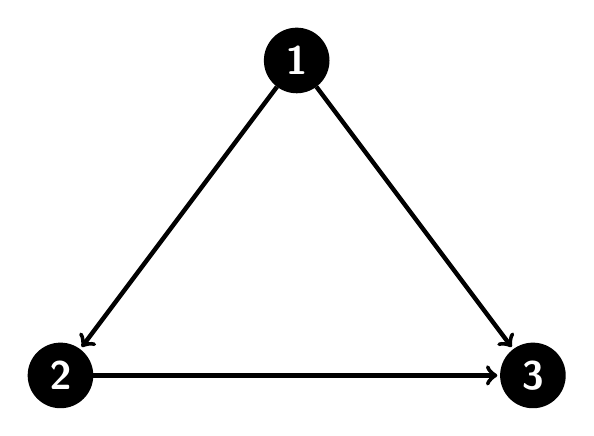
\begin{tikzpicture}[shorten >=1pt, auto, node distance=3cm, ultra thick]
		\tikzstyle{node_style} = [circle,draw=black,fill=black,font=\sffamily\Large\bfseries,text=white]
		\tikzstyle{edge_style} = [draw=black, line width=2, ultra thick,->]
		\node[node_style] (v1) at (0,2) {1};
		\node[node_style] (v2) at (-3,-2) {2};
		\node[node_style] (v3) at (3,-2) {3};
		\draw[edge_style] (v1) edge (v2);
		\draw[edge_style] (v1) edge (v3);
		\draw[edge_style] (v2) edge (v3);
		\end{tikzpicture}
		\caption{Ejemplo de grafo dirigido.}
	\end{figure}	
	
	\item Grafo ponderado: es un grafo que asocia un número real (peso o ponderación) a cada arista. Estos grafos se suelen aplicar a problemas de optimización como por ejemplo para hallar el camino más corto.
	
		\begin{figure}[H]
			\centering
			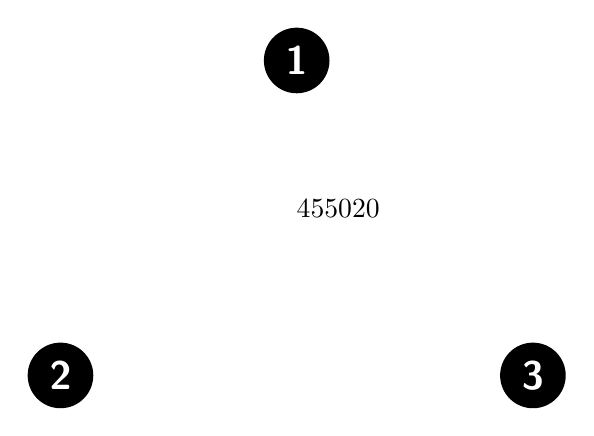
\begin{tikzpicture}[shorten >=1pt, auto, node distance=3cm, ultra thick]
			\tikzstyle{node_style} = [circle,draw=black,fill=black,font=\sffamily\Large\bfseries,text=white]
			\tikzstyle{edge_style} = [draw=black, line width=2, ultra thick,->]
			\node[node_style] (v1) at (0,2) {1};
			\node[node_style] (v2) at (-3,-2) {2};
			\node[node_style] (v3) at (3,-2) {3};
			\Edge[label=$45$](v1)(v2)
			\Edge[label=$50$](v1)(v3)
			\Edge[label=$20$](v2)(v3)
			\end{tikzpicture}
			\caption{Ejemplo de grafo ponderado.}
		\end{figure}

\end{itemize}

\newpage

\section{Representación de grafos}

Además de la geométrica, existen diferentes formas de representar un grafo, vamos a ver algunas formas alternativas que nos pueden ser útiles para almacenarlos en un computador. 

\begin{figure}[H]
	\centering
	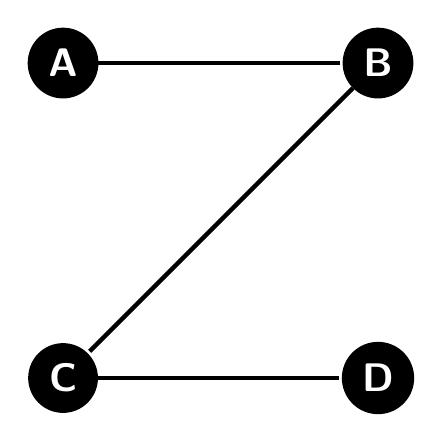
\begin{tikzpicture}[shorten >=1pt, auto, node distance=3cm, ultra thick]
	\tikzstyle{node_style} = [circle,draw=black,fill=black,font=\sffamily\Large\bfseries,text=white]
	\tikzstyle{edge_style} = [draw=black, line width=2, ultra thick]
	\node[node_style] (A) at (-2,2) {A};
	\node[node_style] (B) at (2,2) {B};
	\node[node_style] (C) at (-2,-2) {C};
	\node[node_style] (D) at (2,-2) {D};
	\draw[edge_style] (A) edge (B);
	\draw[edge_style] (B) edge (C);
	\draw[edge_style] (C) edge (D);	
	\end{tikzpicture}
	\caption{Ejemplo de grafo.}
	\label{fig:graphrep}
\end{figure}

\begin{itemize}
	\item Lista de adyacencia: cada vértice tiene una lista asociada con los vértices adyacentes a él. En grafos no dirigidos se produce redundancia.\\
	La lista de adyacencia asociada al grafo \ref{fig:graphrep} es $\{\{B\},\{A,C\},\{B,D\},\{C\}\}$.
	\item Lista de grados: es una secuencia de números, que se corresponden con los grados de los vértices del grafo.\\
	La lista de de grados asociada al grafo \ref{fig:graphrep} es $\{2,2,1,1\}$.
	
	\item Matriz de adyacencia: el grafo está representado por una matriz cuadrada $M_{nxn}$, donde $n$ es el número de vértices del grafo. Si hay una arista entre un vértice $v_{i}$ y un vértice $v_{j}$, entonces el elemento $m_{i,j}$ toma el valor 1, si no toma el valor 0. En el caso de grafos simples la diagonal principal estará formada por ceros.\\
	La matriz de adyacencia asociada al grafo \ref{fig:graphrep} es
	\renewcommand{\kbldelim}{(}
	\renewcommand{\kbrdelim}{)}
	\[\kbordermatrix{
		& A & B & C & D\\
		A & 0 & 1 & 0 & 0\\
		B & 1 & 0 & 1 & 0\\
		C & 0 & 1 & 0 & 1\\
		D & 0 & 0 & 1 & 0
	}.
	\]
	
	\item Matriz de incidencia: el grafo está representado por una matriz $M_{mxn}$, donde $m$ es el número de vértices y $n$ el número de aristas del grafo. Si el vértice $v_{i}$ y la arista $e_{j}$ están conectados, entonces el elemento $m_{i,j}$ toma el valor 1, si no toma el valor 0.\\
	La matriz de incidencia asociada al grafo \ref{fig:graphrep} es
	\renewcommand{\kbldelim}{(}
	\renewcommand{\kbrdelim}{)}
	\[\kbordermatrix{
		& ab & bc & cd\\
		A & 1 & 0 & 0\\
		B & 1 & 1 & 0\\
		C & 0 & 1 & 1\\
		D & 0 & 0 & 1
	}.
	\]
	
\end{itemize}


	
\newpage

\section{Teoría de grafos}

Gracias a la teoría de grafos se pueden resolver problemas en áreas muy distintas.  Algunos de sus muchos usos son: modelización de trayectos en redes de transporte en las que nos interesa obtener caminos óptimos aplicando diversos algoritmos como puede ser el de Floyd, en administración de proyectos se utilizan técnicas como la de revisión y evaluación de programas (PERT) en las que se modela utilizando grafos y optimizando los tiempos, en redes sociales para estudiar la influencia de determinadas personas dentro de círculos de gente, en biología y ecología se aplica a redes tróficas para estudiar como afectaría la extinción de algunas especies a todo el hábitat, etc.\\

\begin{figure}[H]
	\centering
	\subfloat[Prb. Puentes de Königsberg]{
		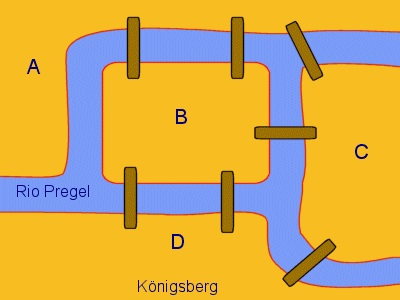
\includegraphics[width=0.3\textwidth]{images/aplicaciones1.jpg}}
	\subfloat[Plano de metro]{
		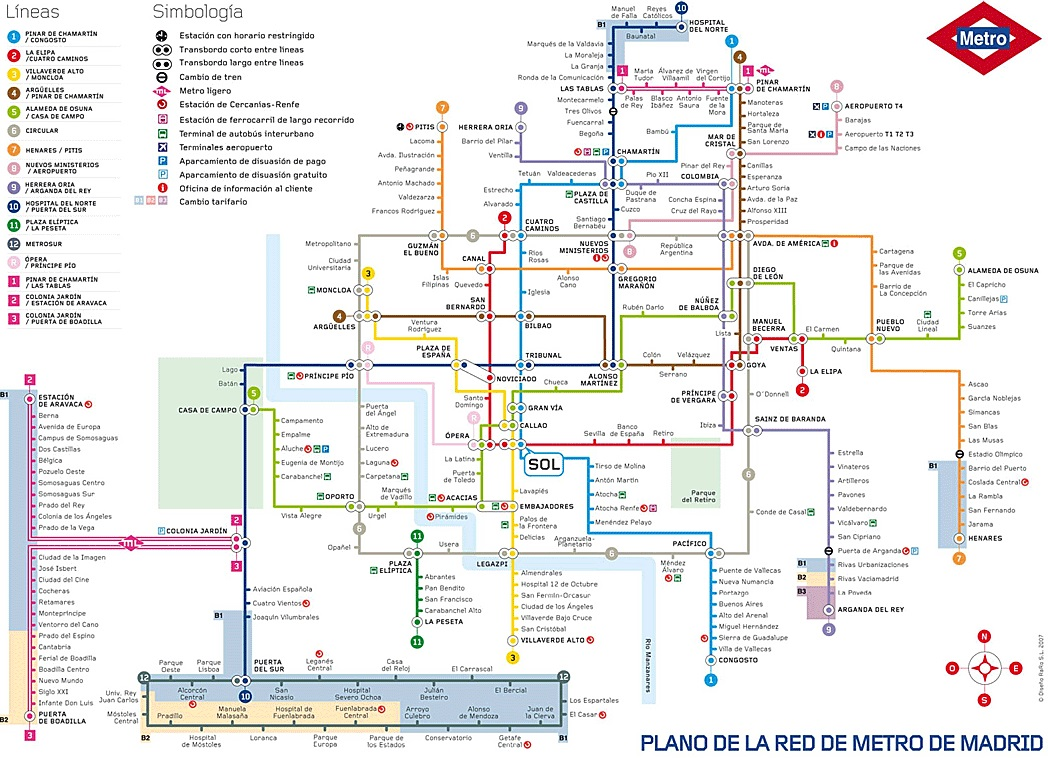
\includegraphics[width=0.3\textwidth]{images/aplicaciones2.jpg}}
	\subfloat[Moléculas]{
		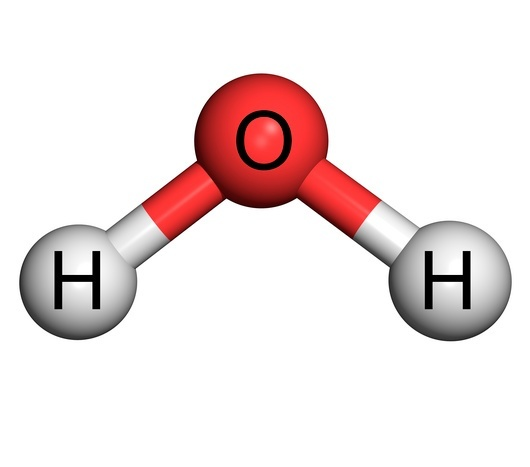
\includegraphics[width=0.3\textwidth]{images/aplicaciones3.jpg}}\\
	\subfloat[Red de computadoras]{
		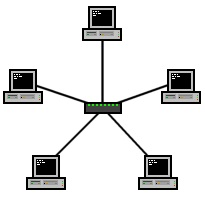
\includegraphics[width=0.3\textwidth]{images/aplicaciones4.jpg}}
	\subfloat[Cadena trófica]{
		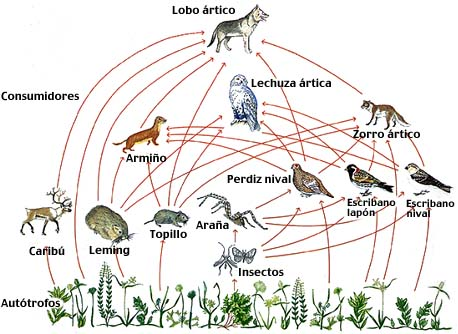
\includegraphics[width=0.3\textwidth]{images/aplicaciones5.jpg}}
	\subfloat[Redes sociales]{
		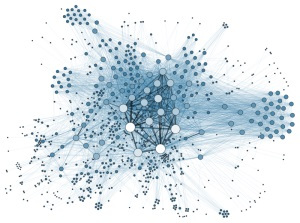
\includegraphics[width=0.3\textwidth]{images/aplicaciones6.jpg}}\\
	\subfloat[Teo. seis grados de separación]{
		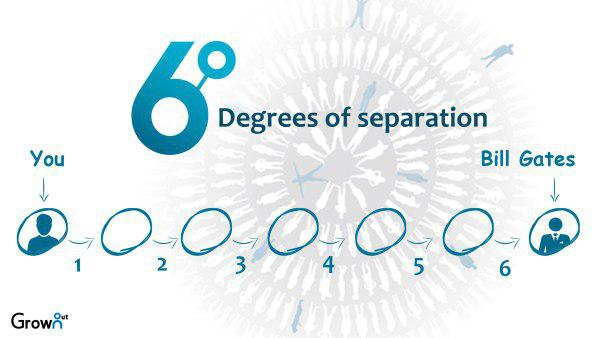
\includegraphics[width=0.3\textwidth]{images/aplicaciones7.jpg}}
	\subfloat[Prb. Coloreado de mapas]{
		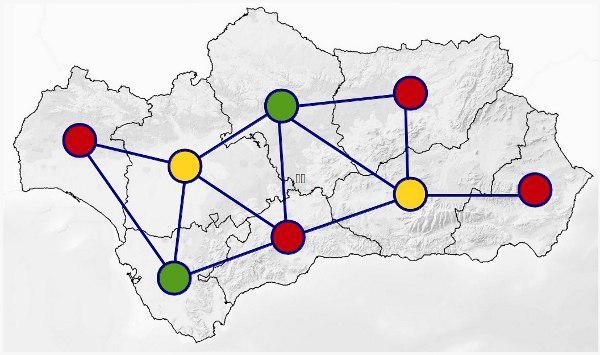
\includegraphics[width=0.3\textwidth]{images/aplicaciones8.jpg}}
	\subfloat[Diagrama de PERT]{
		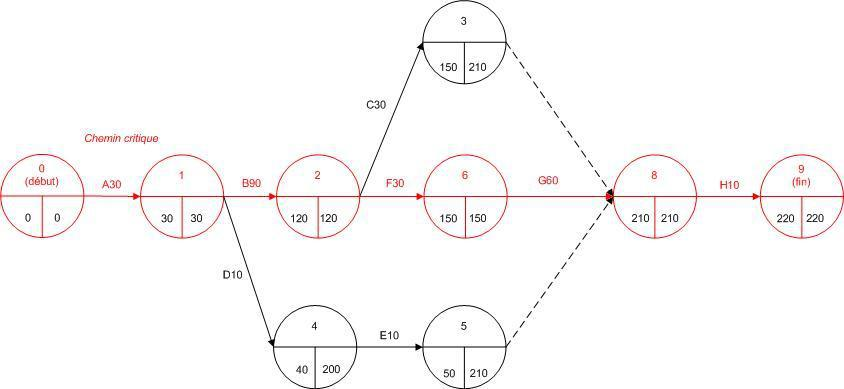
\includegraphics[width=0.3\textwidth]{images/aplicaciones9.jpg}}	
	\caption{Múltiples aplicaciones de teoría de grafos.}
\end{figure}
